\documentclass{article}

%----------------------------------------------------------------------------------------
%	PACKAGES AND OTHER DOCUMENT CONFIGURATIONS
%----------------------------------------------------------------------------------------

\usepackage[T1]{fontenc}
\usepackage[utf8]{inputenc}
\usepackage{lmodern}
\usepackage[english]{babel}
\usepackage[autostyle]{csquotes}
\usepackage{graphicx} % Required for inserting images
\usepackage[hyphens]{url}
\usepackage{hyperref}
\usepackage{amsmath}      % for additional mathematical features
\usepackage{amsfonts}     % for mathbb command
\usepackage{float}
\usepackage{setspace}
\usepackage{listings}
\usepackage{rotating}
\doublespacing
\usepackage[backend=biber,style=authoryear]{biblatex}
\renewcommand*{\bibfont}{\small}
\addbibresource{Bibliography.bib}
\usepackage{tcolorbox}
\usepackage{amssymb}

%----------------------------------------------------------------------------------------
%	DOCUMENT MARGINS
%----------------------------------------------------------------------------------------

\usepackage{geometry} % Required for adjusting page dimensions and margins

\geometry{
	paper=a4paper, % Paper size, change to letterpaper for US letter size
	top=3cm, % Top margin
	bottom=3cm, % Bottom margin
	left=3cm, % Left margin
	right=3cm, % Right margin
	headheight = 10pt, % Header height
	footskip = 1.5cm, % Space from the bottom margin to the baseline of the footer
	headsep = 1.2cm, % Space from the top margin to the baseline of the header
	%showframe, % Uncomment to show how the type block is set on the page
}

%----------------------------------------------------------------------------------------
%	SECTION TITLE APPEARANCE
%----------------------------------------------------------------------------------------


\title{Diversity as a management tool for forest ecosystem \\ 
\large A theoretical exploration using control theory and viability analyses}
\author{Clementine de Montgolfier}
\date{Dec 2023}

\begin{document}

\maketitle

\section{Summary}

Defining optimal forest management strategies in a changing world is a challenge in the field of forest ecology. The complexity of forest ecosystems, coupled with the uncertainty of future climate conditions, makes it difficult to determine the best course of action. The concept of forest diversity is a key consideration in this debate, as it is believed to be a significant factor in the resilience of forest ecosystems. This study aims to explore whether diversity can be used as a management tool to maintain the ecosystem in a desirable state. To this end, we will use a theoretical model of a mixed-species, multi-layered forest, and apply control theory and viability analyses to assess the relationship between diversity and management trajectories, considering both species and vertical diversity at the stand level. RESULTS\\

\noindent \textbf{Keywords:} forest management, diversity, control theory, viability theory

\section{Intro}

\subsection{State of forest and management practices}

Forest covers 31\% of the territory in France, however forest health metrics show rapid degradation  marked by an alarming +80\% increased mortality rate, a 4\% decline in growth and a deceleration in carbon storage due to the growing number of health crises combined with more frequent droughts ~\autocite{IGN}. This impacts forest composition, structure, dynamics and the provisioning of ecosystem services to human populations (Climate regulation, water purification, wood production, air quality, cultural leisure...) ~\autocite{grammatikopoulouValueForestEcosystem2021}. Notably, 94\% of these forests are designated as productive, emphasizing the critical need to adapt management strategies to address these emerging challenges. Managers have engaged adaptative policy actions to robustly sustain the state of these forests. One class of strategy is now frequently compared empirically and with models, involving the adaptation from monospecific forets stand into mixed species stands or uneven forest management, replacing clear-cutting by retention forestry and irregular shelterwood involving a diversity of selectives logging practices or targets  ~\autocite{raymondIrregularShelterwoodSystem2009}. Knowledge of these two practices is still limited but they are already implemented relying on the idea that diversification is a way to increase multiple ecosystem services (foundation of the biodiversity ecosystem functionning research ~\autocite{tilmanBiodiversityPopulationEcosystem1996}). But given the many uncertainties in climate and complex response of forest systems to management actions, as well as the extremely large number of possible strategies of diversification and interests involved, models and decision science should be called upon to assist their design. Particularly to understand the link between climate change, biodiversity, levels of a diversity of ecosystem services and management practices. \\

\subsection{Diverstity and ecosystem funtionning}

Work on composition diversification and its effects is mainly driven by the first work on biodiversity ecosystem functioning (BEF) from grassland studies in the 70's ~\autocite{tilmanBiodiversityPopulationEcosystem1996}.They showed that there was a positive link between biodiversity and ecosystem functioning. But the mechanisms behind this link are still not well understood. Numerous hypothesis were made to explain this link: competitive exclusion, niche complementary, sampling effect, etc. ~\autocite{aliBiodiversityEcosystemFunctioning2023}. This uncertainty makes it difficult to predict the impact of biodiversity loss.
While the hypothesis of BEF relationship, and its relevance is still debated, it fuels an entire segment of research.
The study of BEF in forest is more recent and mainly focused on the link between species diversity and productivity. A positive relattionship has been demonstrated at a global scale ~\autocite{liangPositiveBiodiversityproductivityRelationship2016}, but also in specific forest ~\autocite{morinTreeSpeciesRichness2011,paquetteEffectBiodiversityTree2011,jourdanManagingMixedStands2021}. But the interaction is not positive in every forest type. ~\autocite{forresterReviewProcessesDiversity2016}.
However one of the way to explain the contrasting results could be that the biodiversity-productivity interaction is context dependant. The relationship seems to be mostly positive in harsh climate and low tree density but negative in suitable environment ~\autocite{juckerClimateModulatesEffects2016}.
It is also reductive to consider productivity as the only characteristic of forest ecosystems, and many other should be accounted for : support of habitat and biodiversity, regulation of flood, carbon storage and also cultural and aesthetic values.
All of them might not be impacted in the same way. For example there doesn't seem to be an effect of mixture on other soil biodiversity ~\autocite{korboulewskyHowTreeDiversity2016}.
To have a better understanding of the impact of biodiversity on forest functioning it seems necessary to study multiple functions at the same time. It has been shown that diversity can increase multi-functionality by the jack-of-all-trades \& master of none mechanism ~\autocite{vanderplasJackofalltradesEffectsDrive2016} while not optimizing any of them. With this blindly increasing biodiversity can increase forest multi-functionnality without optimizing any of them and leading sometimes to trade-offs. For instance, tade-offs can be observed in the balance between young and old grown forests, if the former are more productive, they store less carbon than the latter ~\autocite{caspersenSuccessionalDiversityForest2001}. It is thus important to define the functions that we want to preserve as well as threshold for each of them.

Vertical diversity brought back in forest by uneven forest management have also been advocated to be a possible solution to the increasing fralgility of this ecosystem ~\autocite{guldinRoleUnevenAgedSilviculture1996}. Today only 25\% of managed forest in europe is composed of uneven aged stand (foresteurope.org), but the actual effect of such management is hardly consensual. In his review in 2017 Nolet ~\autocite{noletComparingEffectsEven2018} concludes that "overall, the complexity	of comparing even- and uneven- aged silviculture may explain the surprisingly limited number of studies that compare ecological effects of even- and uneven- aged silviculture".

The conclusions drawn, whether related to composition or vertical diversity, are highly dependent on the metric chosen as a proxy for diversity species richness ~\autocite{juckerClimateModulatesEffects2016, guldinRoleUnevenAgedSilviculture1996, noletComparingEffectsEven2018}. This complexity adds an additional layer of intricacy to understanding the connections between these metrics and the potential services the forests could offer. Additionally, the challenge extends to understanding the specific impacts associated with various management practices both directly on diversity and through other avenues, influencing overall forest health. \\

\subsection{Natural and anthropic disturbances for diversity}

Timber extraction stands as an essential component in comprehending the forest ecosystem in France, given that almost all forests are managed for this purpose. Managment can be a way to maintain diversity in forest, by creating gaps and allowing new species to grow. While the primary goal remains the optimization of wood production, numerous new management practices have been devised to foster greater forest diversity.
The literature presents a diversity of perspectives on the relationship between disturbance control and biodiversity. One notable theory in this discourse is Connell's 'Intermediate Disturbance Hypothesis' (\citeyear{connellDiversityTropicalRain1978}). According to Connell, minimal disturbance results in low diversity due to competitive exclusion, while excessive disturbance eliminates species incapable of swift re-colonization. Intermediate disturbance, however, allows for the coexistence of species with different disturbance tolerances, resulting in high diversity. This theory has been widely debated with some studies supporting the hypothesis ~\autocite{sheilDefiningDefendingConnell2013}, others strongly refuting it, even suggesting to abandon it ~\autocite{foxIntermediateDisturbanceHypothesis2013}.
Adding further nuance, considering the identity of species, particularly the focus on dominant species (~\autocite{chessonMechanismsMaintenanceSpecies2000,barabasChessonCoexistenceTheory2018,pichancourtGrowingBiodiverseCarbonrich2014}), play a crucial role in understanding the intricate dynamics of disturbance and its impact on biodiversity.

Forest management encompasses more than just harvesting; it involves considerations such as plantation practices, which can directly address questions related to species choice and turnover in the face of climate change. The intricate dynamics of species selection become a crucial consideration, presenting a potential advantage in the context of forest plantation management (\autocite{brockerhoffPlantationForestsBiodiversity2008}). Furthermore, the exploration extends to the conversion to uneven shelterwood practices, prompting research inquiries into the optimal methodologies involved (\autocite{sinhaOptimalManagementNaturally2017,dudumanForestManagementPlanning2011,nylandEvenUnevenagedChallenges2003}).

These studies emphasize the need for a comprehensive understanding of forest management beyond traditional cutting practices. They strive to provide guidance for managing biological diversity by manipulating disturbance levels, encompassing considerations for both species composition and vertical structure. However extracting an optimal management trajectory proves challenging due to the current limitations in our understanding, coupled with the added complexity of simultaneously maximizing multiple ecological functions. Yet, a significant limitation persists as the primary objective remains wood extraction. Other ecosystem functionalities are often relegated to mere side constraints. Exploring the possibility of manipulating various constraints could open new perspectives on the incidental advantages they may yield.

\subsection{Control theory and viability}

There doesn't seem to be any optimal solution to manage such complicated ecosystems, while taking into account their multi-functionality. Some methods, such as viability theory ~\autocite{aubinStochasticViabilityInvariance1990}, have been developed to actively discover sequences of actions sustaining multiple objectives within satisfaction constraints. Viability analyses establishes a framework to define control and states that can be combined to stay in our biological constraints for as long as needed \autocite{rougeExtendingViabilityTheory2013}.
Viability theory finds application in scenarios where objectives involve ecosystem services in forest social-ecological systems ~\autocite{mathiasUsingViabilityTheory2015, Houballah2021, Houballah2023}. In these studies, biodiversity is leveraged to identify viable control sequences, sustaining forest biodiversity and some ecosystem services through timber extraction control.
Nevertheless, it has not yet been employed to comprehend how controlling species diversity and selective disturbance targets can lead to viable management trajectories.

\subsection{Hypothesis and objectives of the study}

Our main hypothesis is that there exist a viable control law of the diversity level of species or of selective disturbance targets that can respect the constrains on biodiversity and productivity. To test this, we developed a simple theoretical model of multi-species/layers forest ecosystem dynamics. The model was parameterized for two species with different vital rates (growth, survival, reproduction) and competition for light between three vertical storeys (upper, mid, under). The model was used to predict annual Shannon diversity index of species, vertical structure, above-ground biomass, and timber extraction, under all the possible combinations of logging strategies affecting the three species and storeys every five years.  Given the combinations, the algorithm from viability theory were used to deduce the the set of controls (including index of diversity of selective logging targets) that respect our constraints.

\section{Methods}

\subsection{Forest model}

\subsubsection{Choice of model}

Forest models are very diverse, they evolved with need, understanding of ecosystem processes, and technological innovations. They are applied at different spacial scales from tree, to stand to landscape level. They integrate different processes as growth, regeneration, mortality, management, photosynthesis, evapotranspiration, disturbances with more or less details. Numerous types of forest model classification exist ~\autocite{porteModellingMixedForest2002}, but for this short exploration only a simple classification in two groups will be useful ~\autocite{fontesModelsSupportingForest2011} : first there are the empirical models that are developed on experimental data (and then theoretical models which are the continuous equivalent with differential equation), secondly there are the process based models (PBM) that infer dynamics from underlying processes at community,individual or cellular level. 

Amongst PBM, the biggest family is formed by Gap-models ~\autocite{bugmannREVIEWFORESTGAP2001}, built upon the assumption that most of forest dynamic is the result of competition for light.
Although gap models show promise, a significant drawback is their complexity, especially when defining the system state. This complexity surpasses our capacity for analysis. However, it is possible to reduce dimensions (and runtime to 5\%) while making minimal assumptions with model aggregation, achieved through tools like DisCForM and TreeMig \autocite{lischkeAggregationIndividualTrees1998,lischkeTreeMigForestlandscapeModel2006} by height discretization.

On the other hand theoretical models are derived from theoretical considerations, and not from detailed mathematical models of tree population dynamics such as gap models. However both of this approach show a remarkable congruence in their formulation \autocite{bugmannREVIEWFORESTGAP2001}.

The limit of the viability analyses is its computational cost, and the need for a simple model, which means a compromise between complexity and realism. The model had to be simple enough to be sumarized by a small number of state variables, but also complex enough to be able to test different management strategies. We hypothesize that we can use a simple theoretical model to explore the effect of diversity on ecosystem services, and that the some results will then be transferable to more complex models. The advantages of this approach is that we can explore a large range of possibilities and test new hypothesis that could not be tested with more complex models.

For this study the needs for stand-level mixed-species size structured forest with a limited number of state variables and the possibility to apply management strategies, led us to the choice of a theoretical model. The model is based on the work of Kohyama and associates ~\autocite{kohyamaStratificationTheoryPlant2009, kohyamaOnesidedCompetitionLight2012}.

\subsubsection{Model description}

The theoretical model described below comes from the study of multiple articles from Kohyama and associates ~\autocite{kohyamaStratificationTheoryPlant2009, kohyamaOnesidedCompetitionLight2012}.
It is a compartment based model with multi species and multi layers structure Figure ~\ref{fig:fig_model}. The dynamic is influenced by growth, regeneration, mortality as well as competition for light from the layers above. There are some differences between the models present in Kohyama 2009 and 2012, in particular definition of birth and competition. We chose to define birth as in Kohyama 2009 as a negative linear, or Verhulst function (and not as a negative exponential, or Ricker function in Koyama 2012). The only difference is that birth in our study is concidere on independant from the number of adult tree. Even if Kohyama 2009 propose a way to add competition for resources by layers below, we chose a strictly one-sided competition from the above layers as in Kohyama 2012.

\begin{figure}[h]
    \centering
    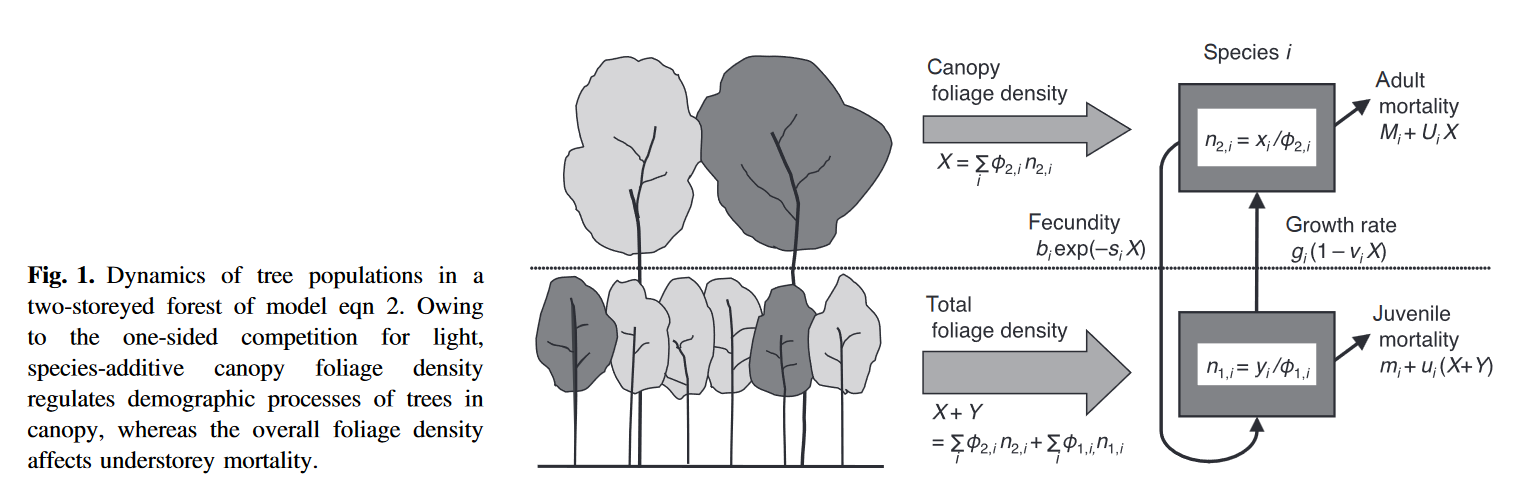
\includegraphics[width=\textwidth]{Figure/Fig_model_Kohyama.png}
    \caption{Figure from ~\autocite{kohyamaOnesidedCompetitionLight2012}}
    \label{fig:fig_model}
\end{figure}

Dynamic of each layer is driven by the competition from above layers foliage density (assimilated to the basal area) $\sum_{i = l}^{L} X_i$ with $X_i$ being the foliage density of layer $i$ :
\begin{equation}
    X_{l} = \sum_{sp} x_{sp,l} = \sum_{sp} \phi_{sp,l} n_{sp,l}
\end{equation}

The various processes are influenced by competition, with a linear negative relationship. Optimal probabilities are determined for each processes (birth $b$, growth $g$ and mortality $m$) without competition. These probabilities are then adjusted based on the process sensitivity ($Cb$, $Cg$, $Cm$) of the layer and species to foliage density.

\noindent The model can be summarised with one differential equation : \\
\begin{equation}\label{eq:model_general}
    \begin{split}
    \frac{dn_{sp,l}}{dt} = & 
    b_{sp,l} (1 - Cb_{sp,l} \sum_{i = 1}^{L} X_{i}) \\
    & + g_{sp,l - 1} \; n_{sp,l-1} (1 - Cg_{sp,l-1} \sum_{i = l-1}^{L} X_{i}) \\
    & - g_{sp,l} \; n_{sp,l} (1 - Cg_{sp,l} \sum_{i = l}^{L} X_{i}) \\
    & - m_{sp,l} \; n_{sp,l}(1 + Cm_{sp,l} \sum_{i = l}^{L} X_{i})
    \end{split}
\end{equation}
\\
And some special cases for lower and upper layers : \\
\begin{center}
    $b_{sp,l} = 0$ for l > 1 \\
    $g_{sp,L} = 0$ \\
    $g_{sp,0} = 0$
\end{center}

Population densities and demographic parameters are defined in ~\ref{tab:coef} and are all positive.

\begin{table}[H]
    \centering
    \begin{tabular}{l l l}
    \hline
    \hline
    \textbf{Abbreviation} & \textbf{Meaning} & \textbf{Unit} \\
    \hline
    \hline
    $l$            & layer index                                                 &          \\
    $L$            & number of layer (i.e. maximum layer)                        &          \\
    $sp$           & species index                                               &          \\
    $SP$           & number of species                                           &            \\
    $n_{sp,l}$     & number of trees of species $sp$ in layer $l$                & $ha^{-1}$  \\    
    $x_{sp,l}$     & foliage density of species $sp$ in layer $l$                & $m^2.ha^{-1}$  \\
    $\phi_{sp,l}$     & mean basal area of tree from species $sp$ in layer $l$    & $m^2$  \\
    $X_{l}$        & foliage density of layer $l$                                & $m^2.ha^{-1}$  \\ 
    $\sum_{i = l}^{L} X_{i}$     & foliage density above layer $l$      & $m^2.ha^{-1}$  \\ 
    $b_{sp}$       & optimal birth rate per tree in layer $L$    &  \\
    $Cb_{sp}$      & birth susceptibility to superior foliage density    & $ha.m^{-2}$           \\
    $g_{sp,l}$     & growth susceptibility to superior foliage density           &  \\
    $m_{sp,l}$     & probability of intrinsic mortality           & \\
    $Cg_{sp,l}$    & growth susceptibility to superior foliage density            &   $ha.m^{-2}$  \\
    $Cb_{sp,l}$    & mortality susceptibility to superior foliage density            & $ha.m^{-2}$    \\
    \hline
    \hline
    \end{tabular}
    \caption{Parameters for the model}
    \label{tab:coef}
\end{table}

\subsubsection{Model parametrisation}

We are starting with a 3 layers 3 species system with a mixture of possible species : \textit{Abies alba}, \textit{Betula pendula}, \textit{Fagus sylvatica}, \textit{Picea abies}, \textit{Pinus sylvestris}, \textit{Quercus pubescens}. The layers are defined by simplifying the IGN (French National Institute for Geographic and Forestry Information) 4-dimensional wood classification used in national forest inventory into 3 classes : dbh (cm) in [0,22.5] for small wood, [22.5,67.5] for medium and large, and [67.5+[ for very large. We have to define all parameters from the model.

Litterature and ForCEEPS simulations where used to adjust the dynamic of the system on a constant climate. (see appendix on parametrisation \autocite{bugmannEcologyMountainousForests1994,morinForestSuccessionGap2021}). Giving the parameters in Table S.\ref{tab:Final_param}.\\
We choose to concentrate our analyses on two species \textit{Abies alba} and \textit{Fagus sylvatica} as their dynamic was the most similar to ForCEEPS (REF to supplementary data) and they can be found together in mixed stand in France.\\

\subsection{Control theory and viability}

Viability theory provides a framework for management of dynamic systems. The challenge lies in finding management strategies (\(u(t)\)) that perpetually keep the system within a space of chosen constraints $K$. Rather than fixating on a single optimal state, the approach is to navigate within a spectrum of acceptable outcomes, preventing irreversible negative impacts.
In our case, the control is discrete and can happen every five years ($\Delta t$), mathematically, this is articulated as a controlled discrete-time dynamical system:

\[
N(t+\Delta t) = g(N(t), u(t), \Delta t),
\]

where \(N(t)\) is the system state at time \(t\), \(u(t)\) is the control applied at time \(t\), and \(g\) is the state transition function. In our case the state of the system, \(N(t)\), is defined by the matrix of the number of trees in each layer and for each species: \[ N(t) = [n_{sp,l}(t)]_{SP \times L} \]. And the state transition function is defined as the cut at discrete time t (\(u(t)\)) and the dynamic following it (described in Equation \eqref{eq:model_general}). The space of possible control is defined by the number of trees that are going to stay after a cut in the two higher layer :

\[
     U = \{u \in \mathbb{N}^{sp*Ncut} \mid \forall sp \in \mathbb{N}_{[1,SP]} \; \& \; l \in \mathbb{N}_{[c,L]}, u_{sp,l} \leq n_{sp,l}\}
\]

The space of possible control is then all the possible compositions of cut layers ($Ncut$ being the number of layers that are cut, 2 in our study, then the first layer cut is $c = L-Ncut+1 = 2$) such as the number of trees left is inferior to the number of trees present before the cut in the layer.\\

The resulting viability kernel (Viab(K)Viab(K)), which includes states where a management strategy can keep the system within desirable states, is formally described as:

\[
Viab(K) = \{N_0 \in K \mid\exists u(\cdot), \forall t \in \mathbb{N}_5, N(t) \in K\},
\]

where \(N_0\) denotes an initial state of the system in our constraints $K$. Within the viability kernel, at least one control strategy $u(\cdot)$ can maintain the system in a desirable state $K$. After the delimitation of the viability kernel all viable controls (\(u_v\)) can be determined and analysed.

To approach the viability kernel we used an algorithm inspired by Saint-Pierre (\autocite{saint-pierreApproximationViabilityKernel1994}).

To define the desirable states we chose constraints on wood extraction and diversity. The first one allow to take into account the economic aspect of forest management. The metrics for diversity were included as a way to take into account the diversity aspect of forest management and it's impact on other services. We chose to use the Shannon index as a measure of species and vertical diversity, as it is a common metric in ecology and combine information about diversity and evenness. \\
\\

After defining the viability kernel for : species...
Known limitation of the viability analyses (harware -> perhaps in discussion)
On a machin RAM, turning for blabla time with , code accessible at github; 
Everything ran with R 4 and analyses where also done with R. REF
We got the results :

\end{document}